%
% PKUMpLtX --- A LaTeX document class for 'Modern Physics Laboratory' in PKU based on `revtex4-2`
%
% Please read `README.md' and the template file before using
% 需要确保 font 选项指定的字体已安装! 具体参见 `README.md' 的说明.
\documentclass[font=default]{mpltx}
\usepackage{booktabs}  
% 以下至 \begin{document} 都仅是本文件为了方便额外定义的命令, 写报告时不需要.
\hypersetup{colorlinks=true}% 超链接带颜色
\usepackage{xcolor}
\newcommand{\note}[1]{{\color{gray}#1}}
\NewDocumentCommand{\pkg}{s o m}{%
    \IfBooleanF{#1}{%
        \IfNoValueTF{#2}%
            {\href{https://www.ctan.org/pkg/#3}}%
            {\href{https://www.ctan.org/pkg/#2}}%
    }%
    {\textsf{#3}}%
}
\newcommand*\cs[1]{\texttt{\textbackslash #1}}
\newcommand*\env[1]{\textit{\texttt{#1}}}
\newcommand*\code[1]{\texttt{#1}}
\newcommand*\file[1]{\textbf{\texttt{#1}}}
\makeatletter
\newcommand\releasedate{%
    \href{https://github.com/CastleStar14654/PKUMpLtX/releases/tag/\mpltx@fileversion}%
        {\mpltx@filedate, \mpltx@fileversion}}
\makeatother
% 以上是本文件为了方便额外定义的命令, 写报告时不需要.

\begin{document}

\title{康普顿散射} % 切合报告内容, 简短明确, 可以不同于讲义
\author{郑熔} % 这里 \emailphone 一定要紧跟在 \author 后方
\emailphone{2300011359@stu.pku.edu.cn}{(86)19805861588}
% 如果改用 \email 则仅需要邮箱参数
\affiliation{北京大学物理学院\quad 学号: 2300011359}
% % 可以使用 \zhdate 自动生成中文日期, 如
\date{\zhdate{2025/10/29}}
% % 也可使用 babel 的 \localedate, 如
% \date{\localedate{2020}{12}{1}}
% % 两者均会输出 `2020 年 12 月 1 日'
% 下面的 \date 的参数是为了自动输出正确版本号, 正式报告请替换为上面的两种 \date 之一
% \date{\releasedate}
\begin{abstract}
  康普顿效应是指入射光子与物质原子中的核外电子产生非弹性碰撞而被散射的过程。
  本实验用 NaI (Tl) 闪烁谱仪, 首先利用$^{137}Cs$和$^{60}Co$的光电峰峰位标定了能量刻度,再测量各散射角的散射 \gamma 光子能谱,由光电峰峰位和光电峰面积得出散射 \gamma 光子能量 h\nu', 并计算出微分散射截面的相对值$\frac{d\sigma(\theta)}{d\Omega}/\frac{d\sigma(\theta_0)}{d\Omega}$.
  将理论值与实验值进行对比,验证了实验的正确性。
  % \note{本文档为对 \href{https://github.com/CastleStar14654/PKUMpLtX}{\pkg*{PKUMpLtX}} 的使用示例, 灰色部分为额外针对 \LaTeX{} 模板使用的说明或是一些能提升输出效果的琐碎细节.
    % 也请注意查看源文档 \file{template.tex} 中的注释.}
\end{abstract}
\keywords{康普顿效应,散射截面}

\maketitle

\section{引言}
康普顿的X射线散射实验证实了光子是具有能量 $E = \hbar \omega$和动量$p=\hbar k$的粒子。因此,在光子和电子等微观粒子相互作用的过程中,能量守恒和动量守恒依然成立。

我国物理学家吴有训先生在康普顿先生的指导下对康普顿效应在理论和实验上均进行了验证,这大大加快了大家对康普顿效应的认识。

本实验通过使用康普顿散射仪,对能量刻度进行了标定,并验证了康普顿散射的\gamma 光子能量能量和微分散射截面以及散射角的关系。

\section{理论}
康普顿效应是指入射光子与物质原子中的核外电子产生非弹性碰撞而被散射的过程。碰撞时,入射光子把部分能量转移给电子,使他脱离原子成为反冲电子。同时,散射光子的能量和运动方向发生变化。
如\autoref{fig:lilun}所示,经过一系列的推导可以得出:
$$ 
h\nu' = \frac{h\nu}{1 + \frac{h\nu}{m_0 c^2}(1 - \cos\theta)}
$$
\begin{figure}
  \centering
  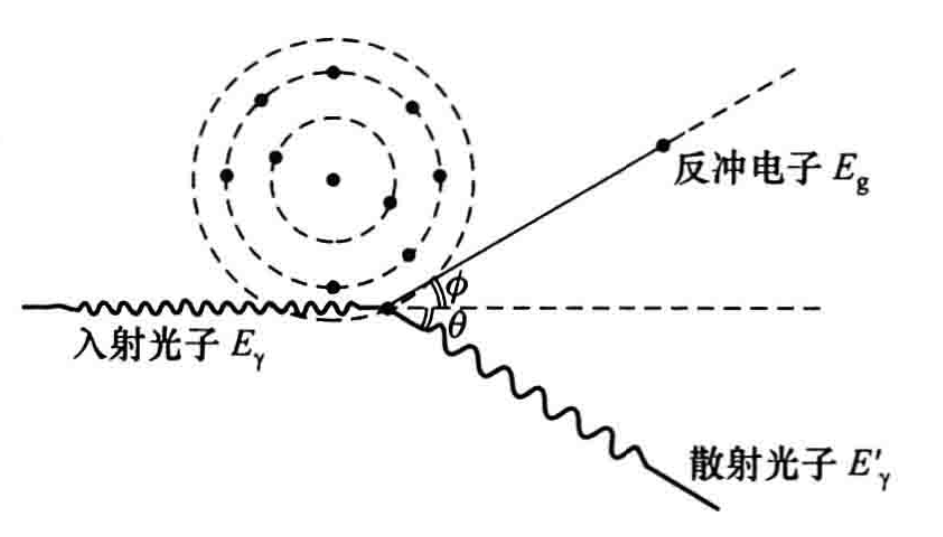
\includegraphics[width=0.85\linewidth]{fig/lilun.png}
  \caption{康普顿散射实验示意图}
  \label{fig:lilun}
\end{figure}
  
康普顿散射的微分界面满足克莱因-仁科公式:
$$ 
\frac{\mathrm{d}\sigma(\theta)}{\mathrm{d}\Omega} = r_0^2 \left[ \frac{1}{1 + \alpha(1 - \cos\theta)} \right]^2 \left[ \frac{1 + \cos^2\theta}{2} \right] \left[ 1 + \frac{\alpha^2(1 - \cos\theta)^2}{(1 + \cos^2\theta)\left[ 1 + \alpha(1 - \cos\theta) \right]} \right]
$$
本实验所测得的微分散射截面的相对值$\frac{d\sigma(\theta)}{d\Omega}/\frac{d\sigma(\theta_0)}{d\Omega}$满足:
$$
\frac{\mathrm{d}\sigma(\theta)}{\mathrm{d}\Omega} \bigg/ \frac{\mathrm{d}\sigma(\theta_0)}{\mathrm{d}\Omega} = \frac{N_{\mathrm{p}}(\theta)}{R(\theta)\eta(\theta)} \bigg/ \frac{N_{\mathrm{p}}(\theta_0)}{R(\theta_0)\eta(\theta_0)}
$$
其中,$N_{\mathrm{p}}(\theta)$可以由实验测量得到,
而$R(\theta)$和$\eta(\theta)$可以由教材\cite{jindaiwulishiyan}中给出的表格中的数值再经过三次样条插值得到,分别如\autoref{fig:R}和\autoref{fig:eta}所示。

\begin{figure}[htbp]
  \centering
  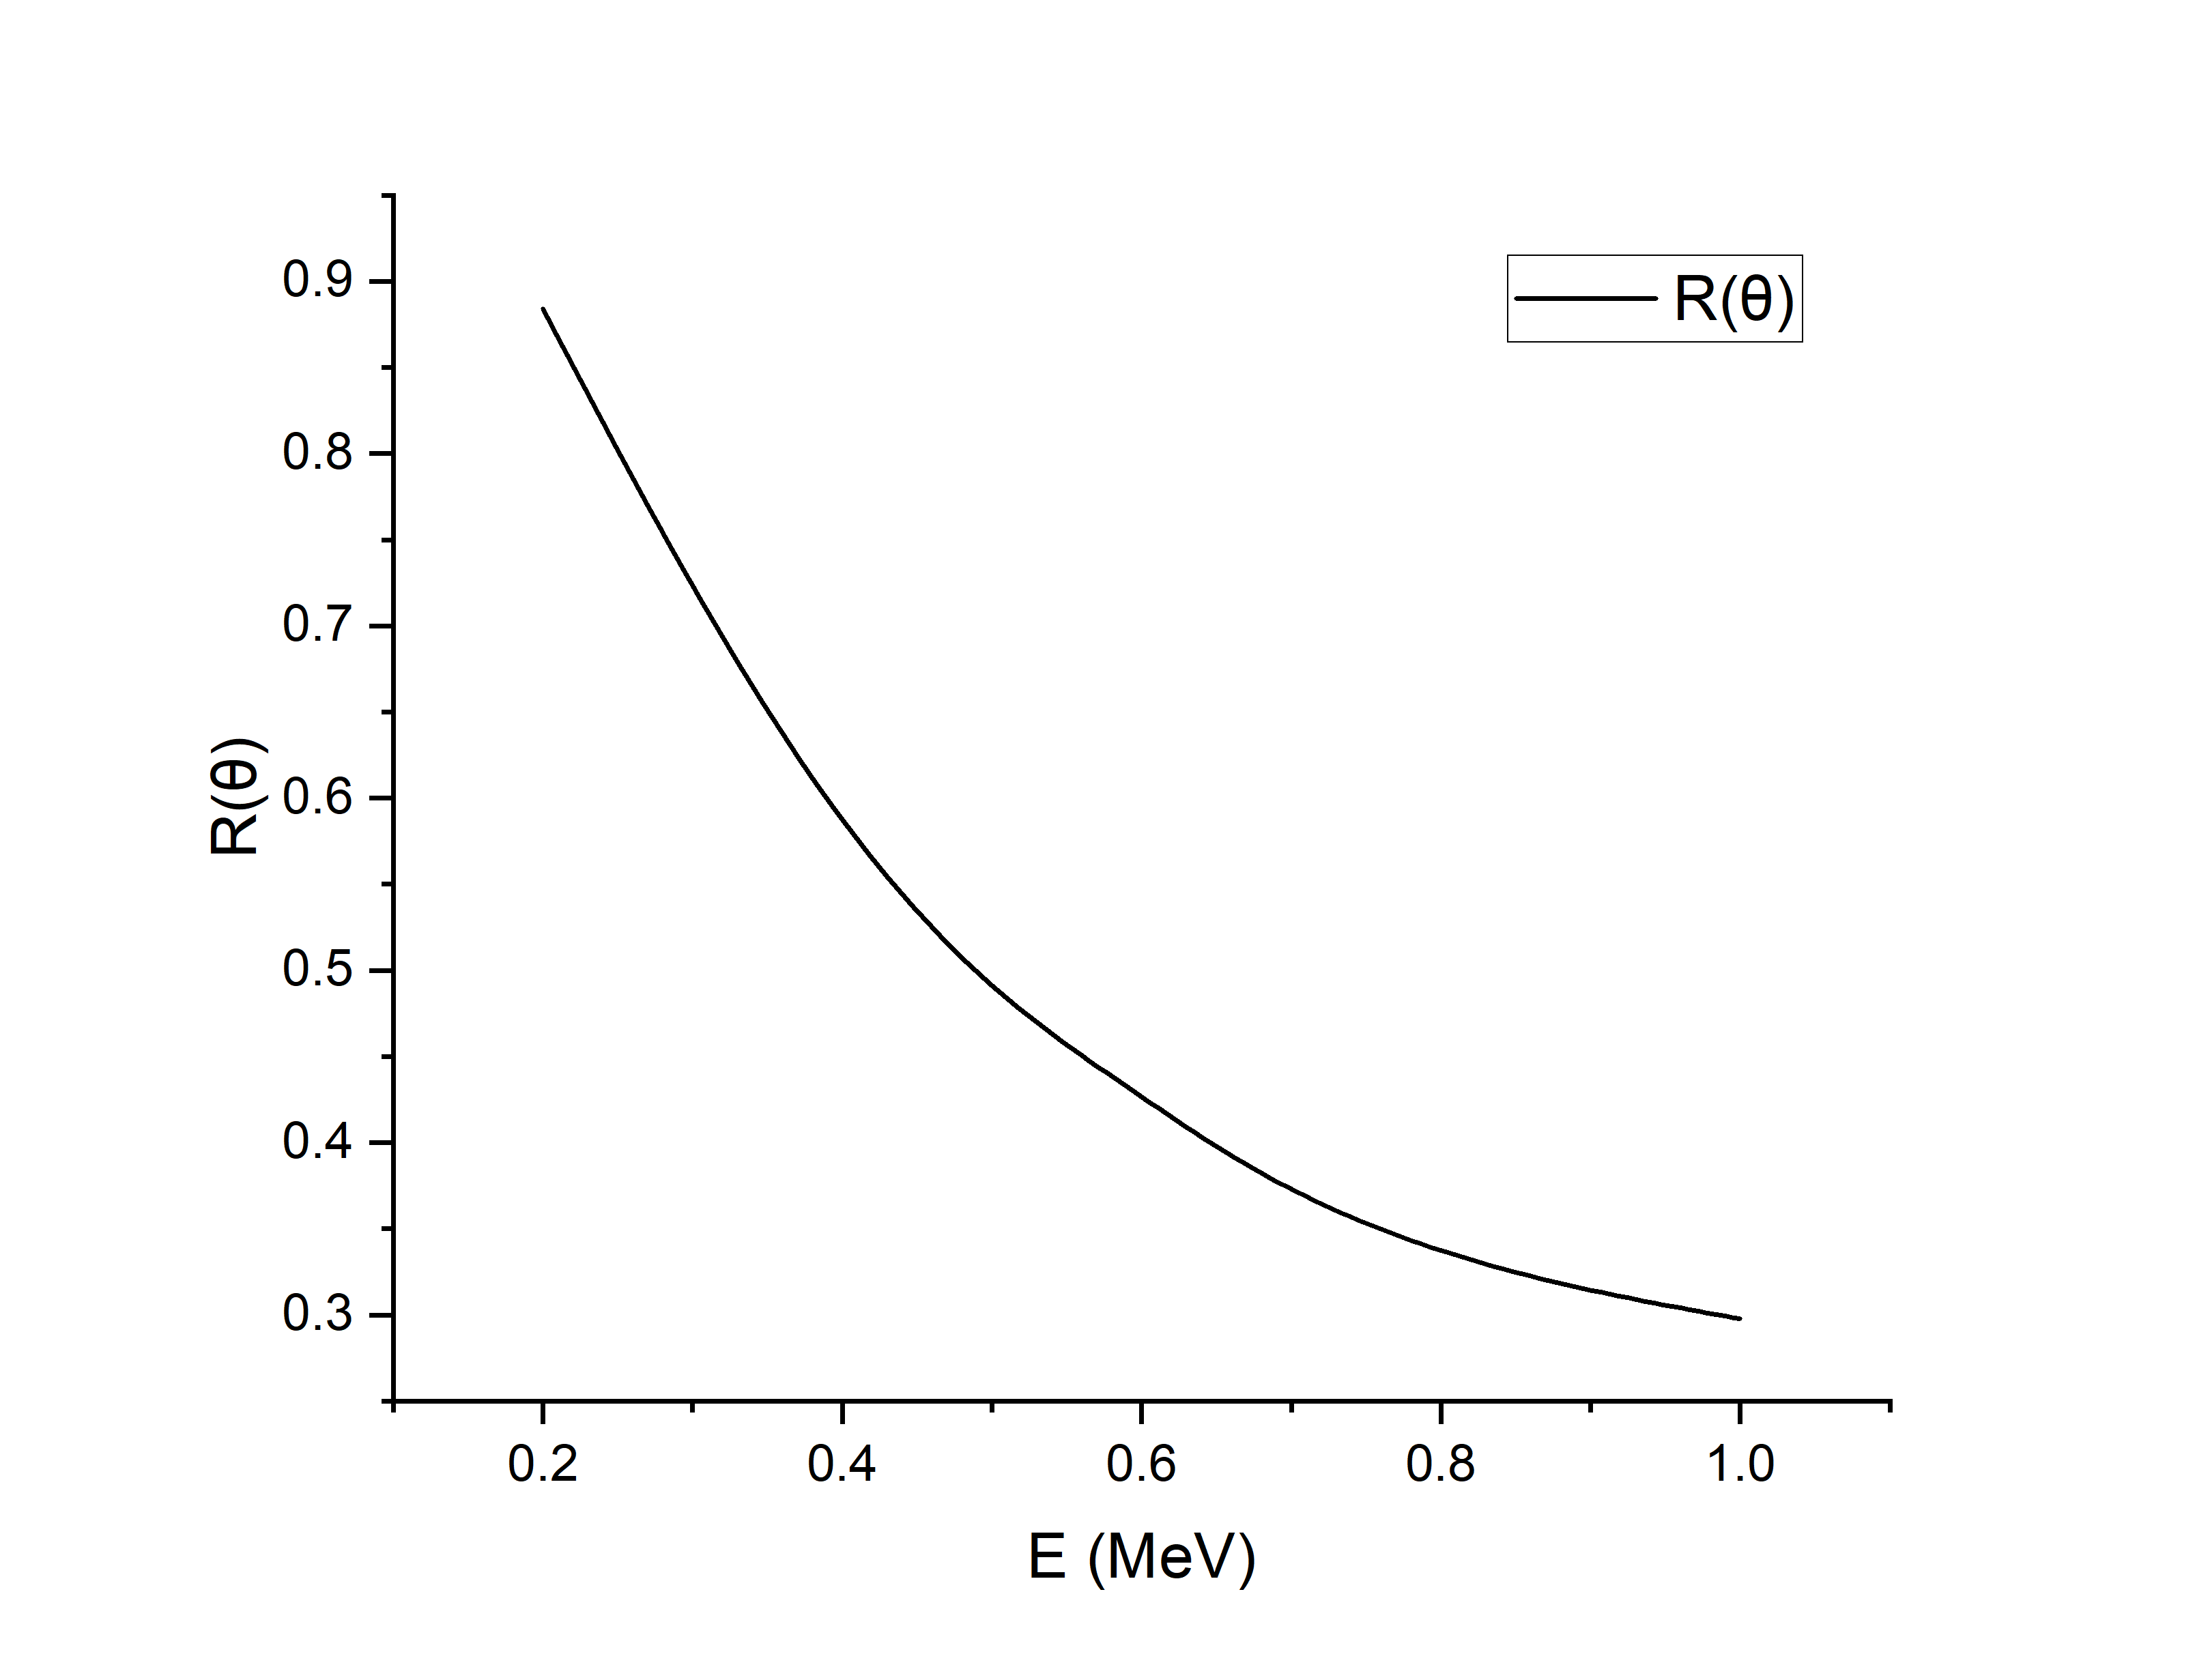
\includegraphics[width=0.85\linewidth]{fig/R.png}
  \caption{$R(\theta)$}
  \label{fig:R}
\end{figure}

\begin{figure}[htbp]
  \centering
  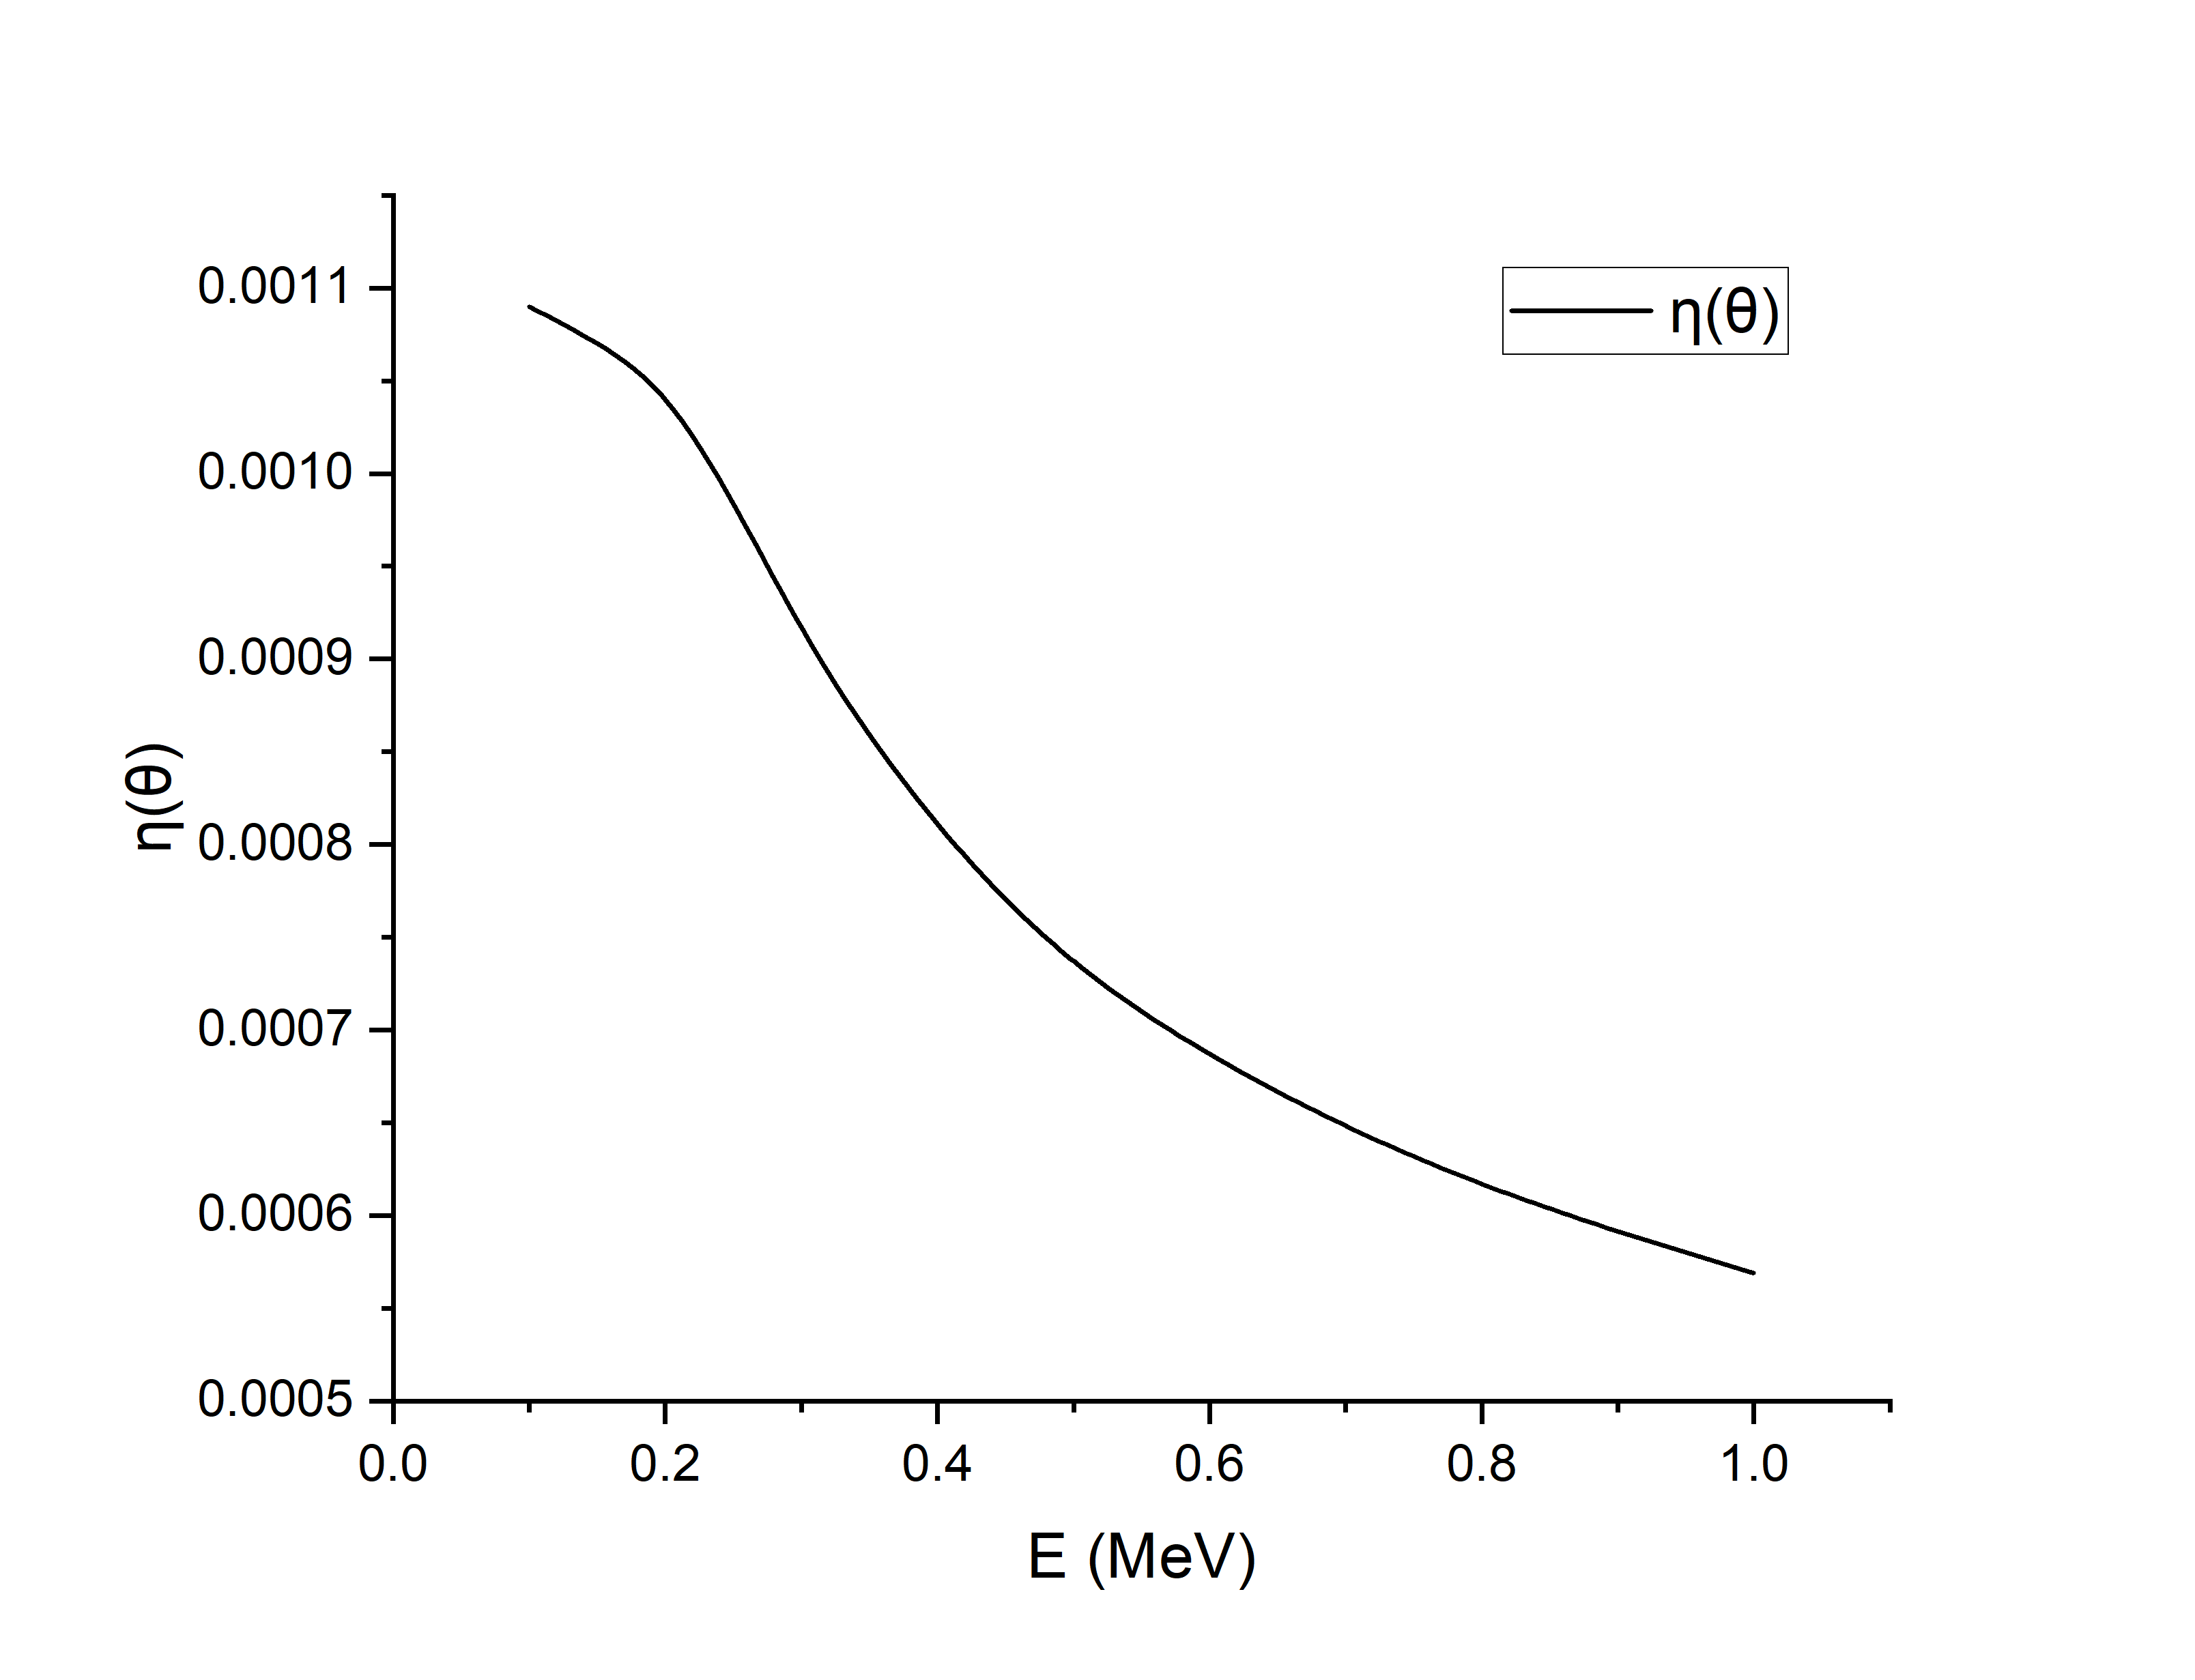
\includegraphics[width=0.85\linewidth]{fig/yita.png}
  \caption{$\eta(\theta)$}
  \label{fig:eta}
\end{figure}

\section{实验}
\subsection{实验装置示意}
实验装置如\autoref{fig:zhaungzhi}所示。

\begin{figure}[htbp]
  \centering
  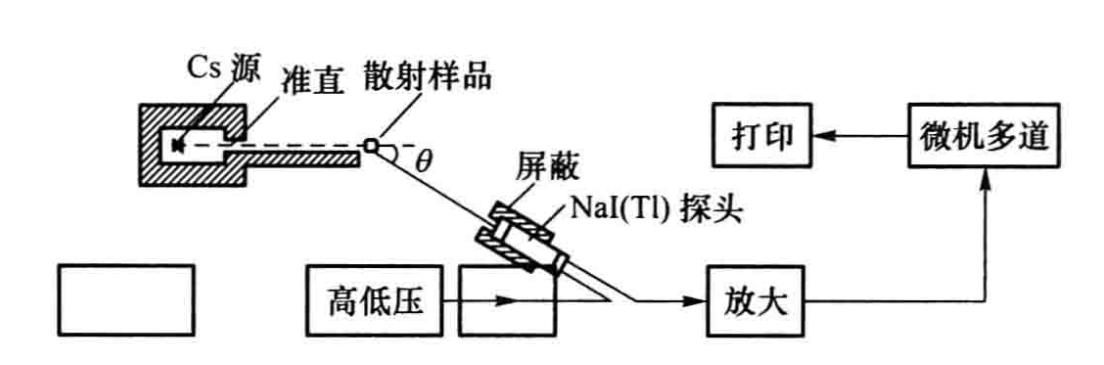
\includegraphics[width=0.85\linewidth]{fig/zhuangzhi.png}
  \caption{康普顿散射实验装置示意图}
  \label{fig:zhaungzhi}
\end{figure}


\subsection{实验步骤}
  \subsubsection{标定能量刻度}
    \begin{enumerate}
      \item 打开${^{137}Cs}$源,将开关打在半开状态,取下散射棒. 调节探头高压$\text{HV=520V}$,预热10分钟. 调节放大$\text{GAIN ADJ} = 3.8$,使得$0.662\text{MeV}$光电峰落在480道左右. 测量其全能谱,通过寻峰定出全能峰对应的准确道数.
      \item 关闭${^{137}Cs}$源,放上${^{60}Co}$,测量其全能谱,定出$1.17\text{MeV}$和$1.33\text{MeV}$两峰对应的准确道数.
      \item 根据测得的三个峰的道址,利用最小二乘法做能量刻度。
    \end{enumerate}

  \subsubsection{康普顿散射峰值和微分截面测量}
    \begin{enumerate}
      \item 安装散射棒,完全打开${^{137}Cs}$源,测量微分散射截面和散射峰能量随散射角的变化. 散射
      角分别取$\theta = 20^\circ,40^\circ ,60^\circ ,80^\circ ,100^\circ ,120^\circ $,对于每个散射角,利用操作
      “寻峰”和“重点区计算”,找出并记录下光电峰的峰位、左右光标道址、重点区总面积. 
      \item 取下散射棒,记录和有散射棒时相同道数区间的面积总计数,从而计算出净峰面积.
      \item 计算散射$\gamma$光子能量和微分散射截面与散射角$\theta$的关系,画出相应关系曲线图,
      并计算实验值和理论值的偏差.在计算过程中,探测器的$R(E), \eta(E)$由 Origin 三次样条插值得到.
    \end{enumerate}

\section{结果及讨论}

  \subsection{实验结果}

    测量${^{137}Cs}$的全谱,通过寻峰定出全能峰对应的道数为 468 . 接着测量${^{60}Co}$的全谱,定出$1.17\text{MeV}$和$1.33\text{MeV}$的对应的道数为$848$和$955$.
    对能量$E$和道数$d$进行最小二乘法拟合$E = a \cdot d + b $,拟合的相关系数为$r = 0.9978$,拟合参数为:
    $$a = 1.36 \times 10^{-3}, \quad b = 2.261 \times 10^{-2}$$

    \begin{figure}[htbp]
      \centering
      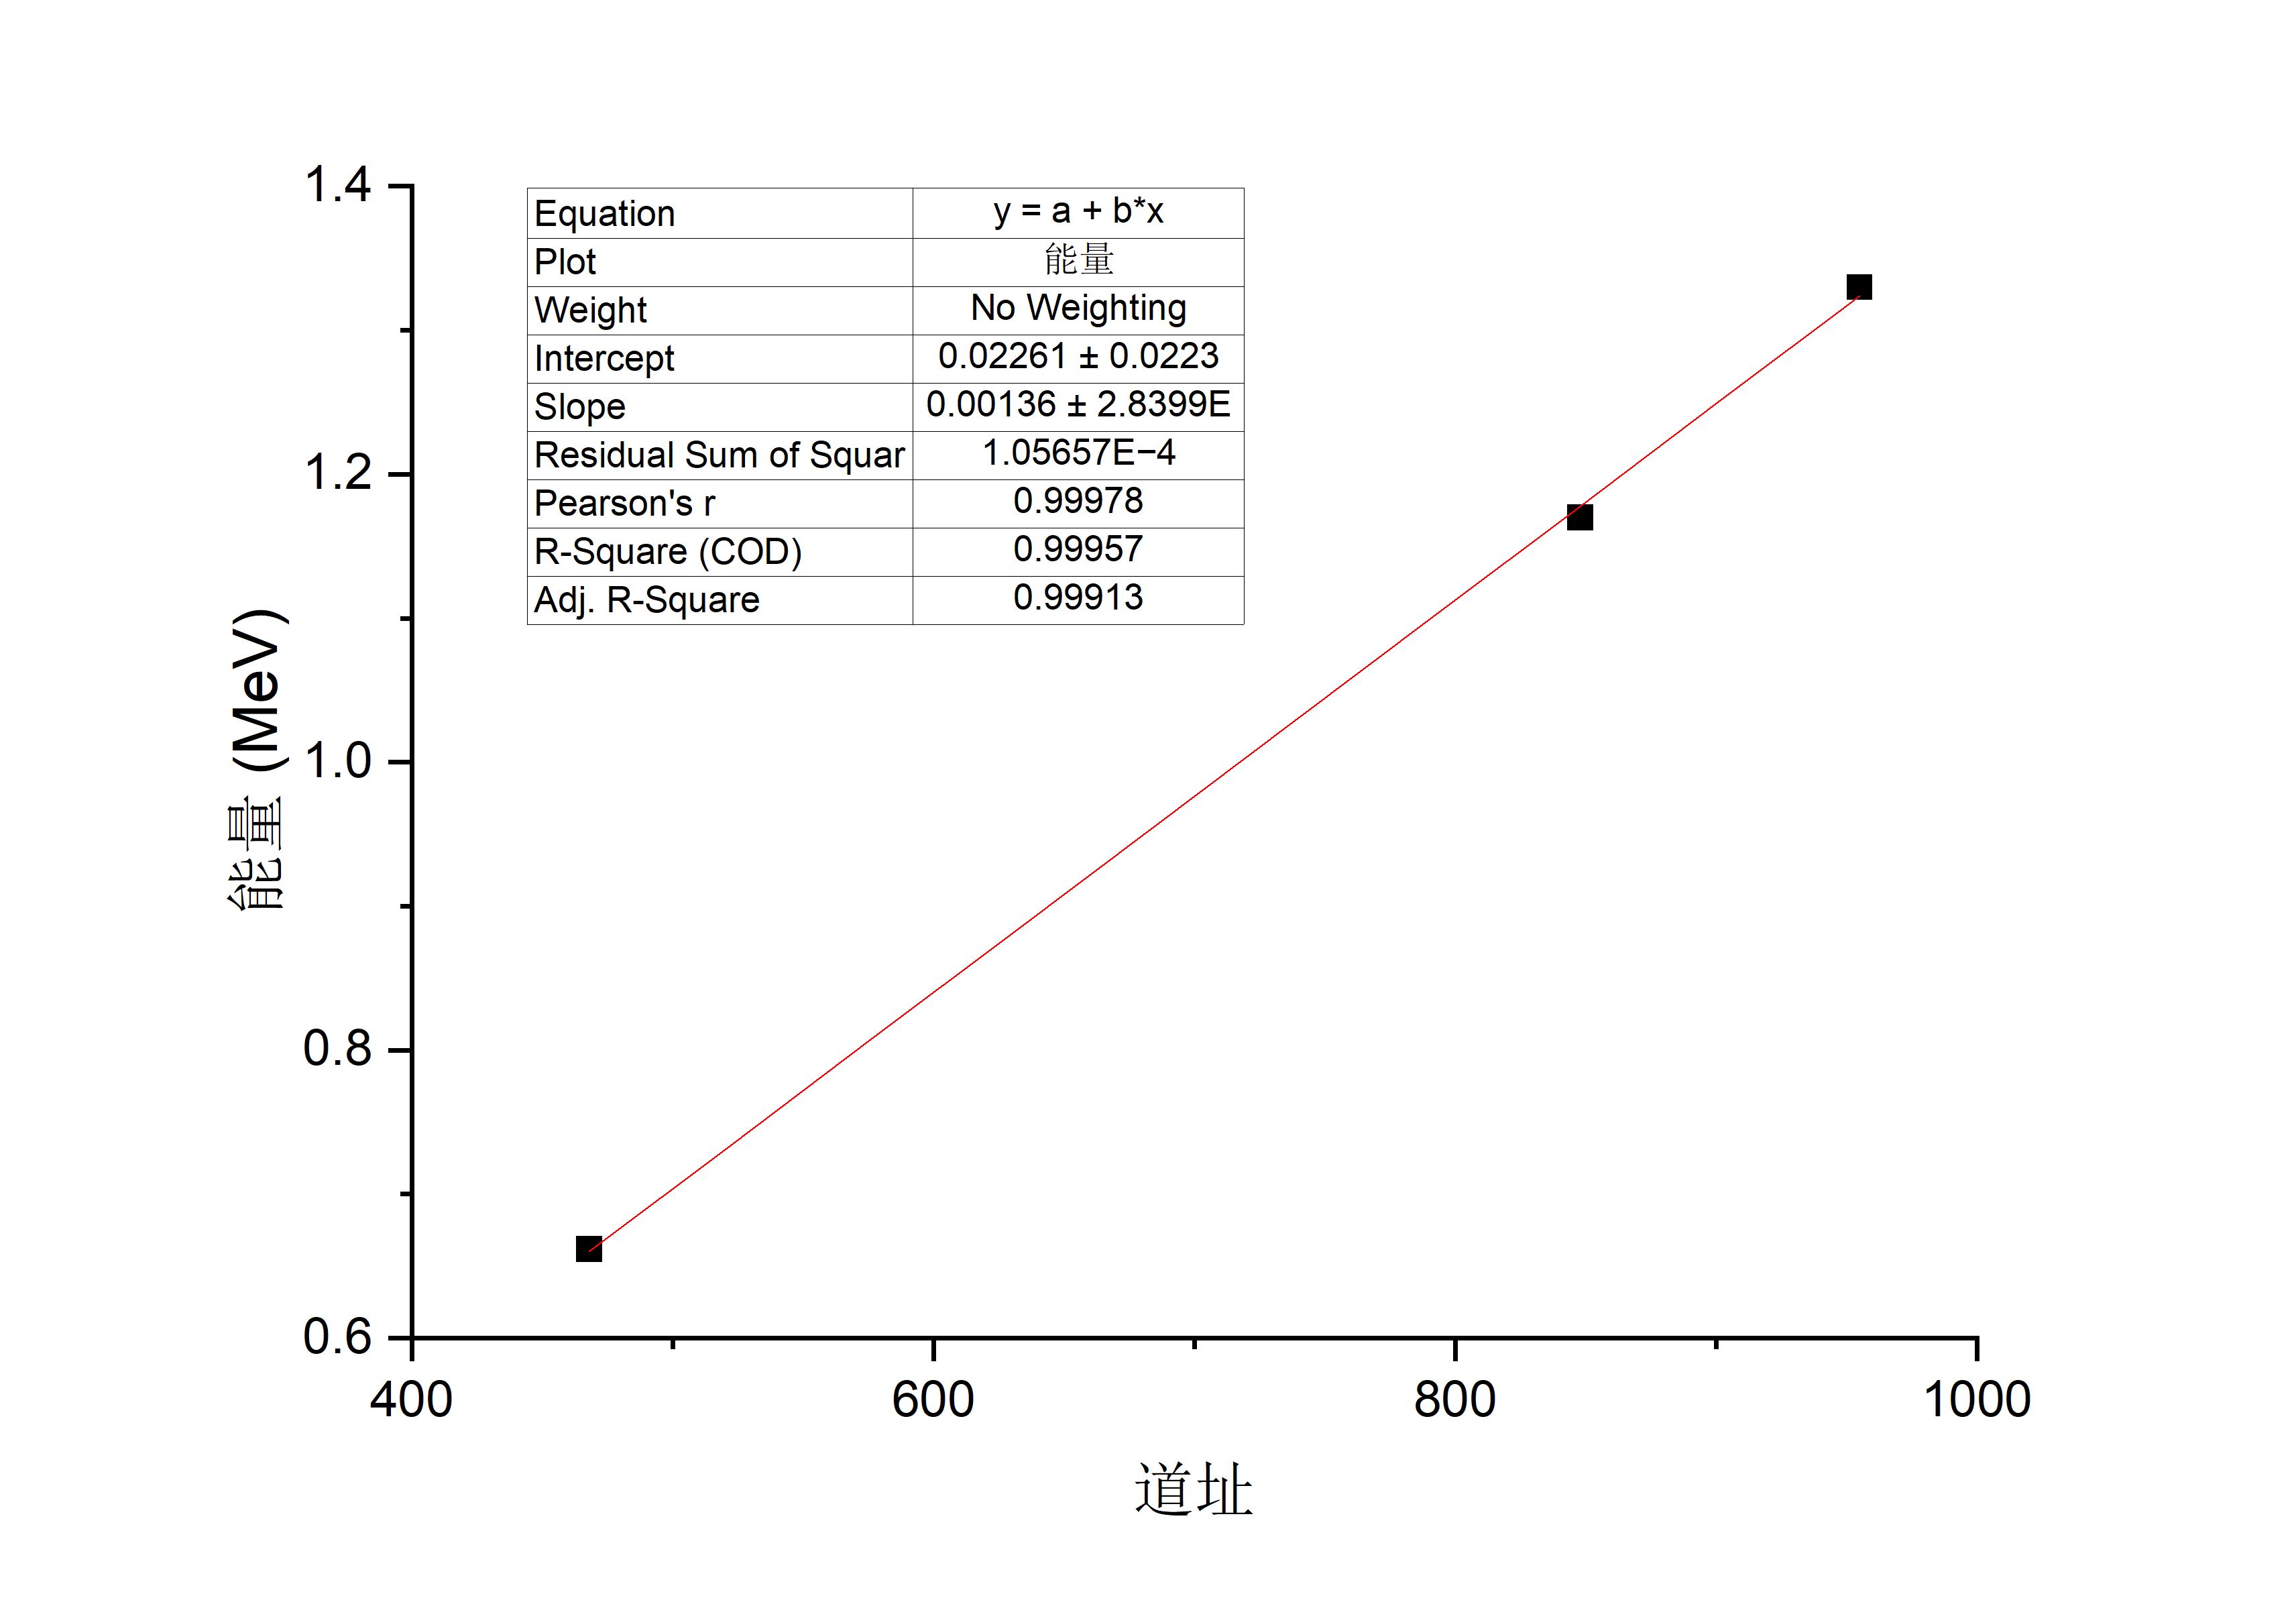
\includegraphics[width=0.85\linewidth]{fig/nihe.png}
      \caption{能量-道址线性刻度}
      \label{fig:nihe}
    \end{figure}

    \subsection{康普顿散射峰值和微分截面测量}

    改变散射角分别对散射信号和本底信号进行测量, 得到的测量结果如\autoref{jiaodu}所示,它是散射信号减去本地信号的画图结果。
    
    得到的结果如\autoref{}所示.

      \begin{figure}[htbp]
        \centering
        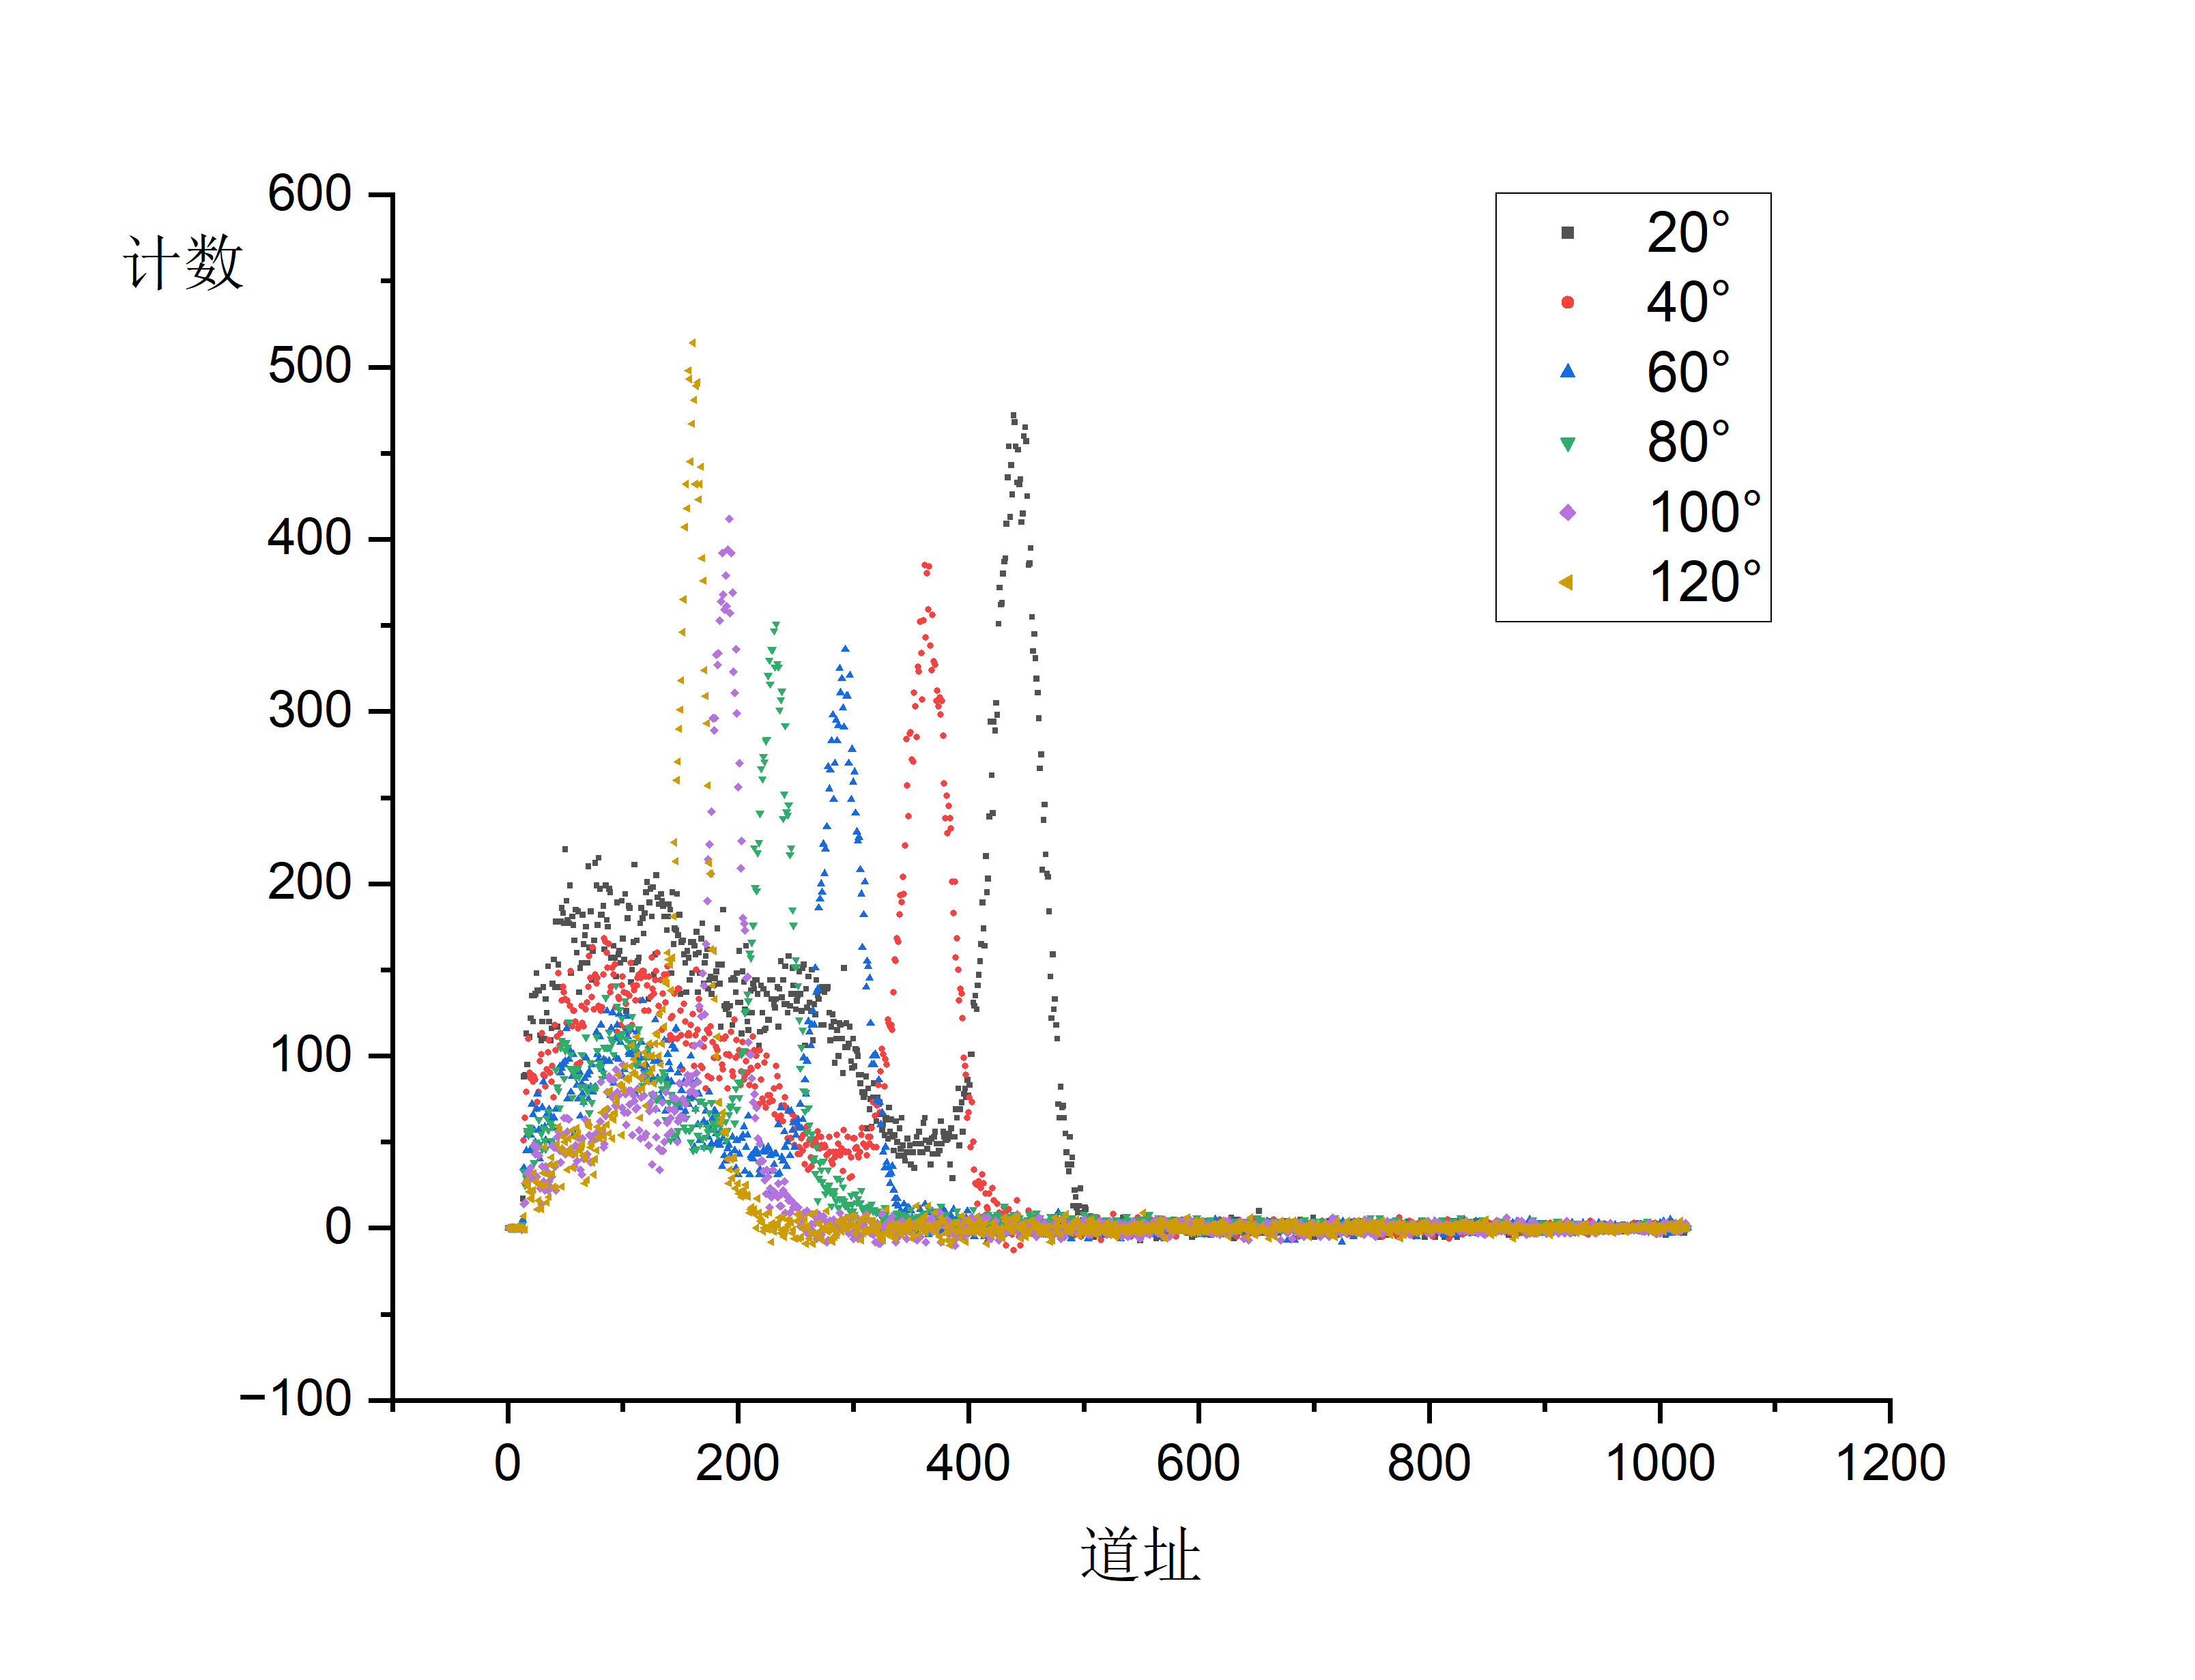
\includegraphics[width=0.85\linewidth]{fig/jiaodu.png}
        \caption{不同角度处的散射能谱}
        \label{fig:jiaodu}
      \end{figure}
      散射峰的能量可以直接利用峰值道址代入此前得到的能量-道址拟合式中得到.
      利用三次样条插值可以得到不同散射能对应的探测器的 $R(E), \eta(E)$ 的大小,
      于是可以得到 $\dfrac{N_p(\theta)}{R(E)\eta(E)}$ 的值,取 $20^\circ$ 时的微分散射截面为基准,
      可以得到不同角度处的相对微分散射截面.将数据处理,得到散射峰能量和相对微分散射截面的大小,并与理论值对比,
      分别如\autoref{tab:gamma_scattering_energy}和\autoref{}所示。
      \begin{table}[htbp]
        \centering
        \caption{散射γ光子能量测量与理论对比数据} % 表格标题(可根据实际需求修改)
        \begin{tabular}{ccccccc}
            \toprule % 顶部粗线(需加载booktabs宏包)
            散射角 $\theta$ ($^\circ$) & 峰位道址 & 能量实验值 (MeV) & $R(\theta)$ & $\eta(\theta)$ & 能量理论值 (MeV) & 能量偏差 (\%) \\
            \midrule % 中间细线(需加载booktabs宏包)
            20 & 447 & 0.63053 & 0.409 & 0.000674 & 0.613735 & 2.66 \\
            40 & 361 & 0.51357 & 0.481 & 0.000729 & 0.507823 & 1.12 \\
            60 & 292 & 0.41973 & 0.565 & 0.000794 & 0.401635 & 4.31 \\
            80 & 232 & 0.33813 & 0.669 & 0.000872 & 0.319645 & 5.47 \\
            100 & 191 & 0.28237 & 0.751 & 0.000940 & 0.262597 & 7.00 \\
            120 & 160 & 0.24021 & 0.818 & 0.000996 & 0.224898 & 6.37 \\
            \bottomrule % 底部粗线(需加载booktabs宏包)
        \end{tabular}
        \label{tab:gamma_scattering_energy} % 表格引用标签(方便文中引用)
      \end{table}



 
\section{结论}
  本实验借助气压扫描式 F-P 标准具, 
  对汞灯 546.1 nm 谱线及其在磁场作用下的塞曼光谱进行观察与测量.
  报告呈现了该谱线在无磁场、0.8 T 磁场 (4 A 励磁电流) 及 1.0 T 磁场 (5 A 励磁电流) 下的光谱图, 
  同时得到了 1.0 T 磁场中 $\pi$ 线和 $\sigma$ 线的光谱. 
  本研究确定了 1.0 T磁场下各子谱线相对于 546.1 nm 谱线的波数差及相对强度, 
  并通过列表与理论值对比, 讨论了产生误差的原因.
  此外, 本研究还对各子谱线波数差进行拟合计算, 得到电子荷质比实验值$1.65 \times 10^{11} C/kg$, 并将其和理论值相比较, 分析了误差产生的原因.

\begin{acknowledgments}
  感谢洪浩老师和助教老师的耐心指导和帮助.
  \par
  感谢搭档王尉丞同学的协助.
\end{acknowledgments}

% bibliography 的参数是你的 *.bib 文件去掉后缀名后的部分
\bibliography{bibli}

\clearpage % 附录前另起一页
\appendix % 附录开始
\section{思考题}\label{app:exercise}


\end{document}
